\chapter{Formal Concept Analysis}
\label{chapter:formal-concept-analysis}

\FCA (FCA) \cite{Wille_Restructuring, WILLE1992493,ganter1999formal} is an approach to reasoning about \textit{concepts} and corresponding \textit{conceptual
structures} in terms of lattice theory and sets. It was first proposed by Wille in his monograph \textit{Restructuring Lattice Theory}
\cite{Wille_Restructuring}, which was an attempt to reestablish a connection between the theory and practice of lattices.

A core aspect of FCA’s foundation is the mathematisation of the philosophical view of concepts, in which a they are understood as a unit
comprising two parts: the \textit{extension}, which is the collection of things said to be instances of the concept, and the \textit{intension},
which contains those properties used to ascribe meaning to the concept \cite{DUQUENNE1999407}.

\section{Basic Notions in Formal Concept Analysis}
\label{section:basic-notions}

Without any formal introduction to this this topic, one can readily grasp the concept of a `person'. We can point to many sense-making properties
of this concept: \textit{mortal}, \textit{warm-blooded}, \textit{mammalian}, and so on. Listing some of the instances included in the extension
of this concept is not particularly challenging either---for example, \textit{the author of this work}, or \textit{the reader}. What is also
clear is that exhaustively specifying a list of either the intension or extension is likely to be a challenging task, even when these lists are
finite, although finiteness need not be a property.

This leads us to what is usually the starting point of FCA a structure called a \textit{formal context}, or simply a context. A context restricts
our ontological consideration to a reduced universe of discourse, as well as detailing the underlying structural relationship that exists
between elements in this universe \cite{Wille_Restructuring,Dau2005}.

\begin{definition}
  \index{formal context} \label{definition:formal-context} A formal context $\context = \GMI$ is a triple comprised of a set $G$ of objects ,
  a set $M$ of attributes, and a binary relation $I \subseteq G \times M$ referred to as an `incidence' relation. For an object-attribute pair
  $(g,m) \in I$ we may say \say{The object $g$ \textit{has} the attribute $m$}.
\end{definition}

We regard the set of objects as being the extensional dimension of the context, while the set of attributes is intensional. However, the
distinction between the extensional and intensional dimensions of the context is largely a matter of convention, or when introducing a FCA a
means of improving intuition. There is no strict requirement around what these sets are made up of, or even that they be distinct, and so it
is perfectly acceptable to have a context where the objects and attributes are the same set; for example, the context
$(\mathbb{N}, \mathbb{N}, \texttt{divides })$ which describes the division relationship between natural numbers.

It should be noted that, while the presence of an object--attribute pair $(g,m)$ in the incidence relation is interpreted as the object
satisfying the respective attribute, FCA is concerned only with \textit{positive} information, and so the absence of a pair in the relation is
not usually interpreted to mean that the object has the negation of the attribute. We will discuss, in more depth, the rather troubling
matter of negation and negative attributes in \Cref{section:contextual-attribute-logic}.

When the cardinalities of $G$ and $M$ are small, contexts may be represented as a cross-table such as in \Cref{cxt:grouplikes}. Each object
is represented by a row in the table, each attribute by a column, and each pair in the incidence relation is marked with an `$\times$' at
the appropriate position \cite[pp. 17]{ganter1999formal}. Given a context presented in this form, it is a trivial task to identify all the
attributes that a particular object satisfies: One need only scan across the respective row and note where the marks appear. The resulting
set of attributes is called the \textit{object's intent}. The dual notion of an \textit{attribute extent} can be found by traversing down a column
in the table.

\begin{figure}[H]
  \centering
  \small
  \begin{cxt}
    \label{cxt:grouplikes} \cxtName{\textbf{\texttt{Algebraic Structures}}} \att{\texttt{closure}} \att{\texttt{associativity}} \att{\texttt{identity}}
    \att{\texttt{inverse}} \att{\texttt{commutativity}} \obj{x....}{\texttt{magma}} \obj{xx...}{\texttt{semigroup}} \obj{xxx..}{\texttt{monoid}}
    \obj{xxxx.}{\texttt{group}} \obj{xxxxx}{\texttt{abelian group}} \obj{x.xx.}{\texttt{loop}} \obj{x..x.}{\texttt{quasigroup}} \obj{.xxx.}{\texttt{groupoid}}
    \obj{.xx..}{\texttt{category}} \obj{.x...}{\texttt{semicategory}}
  \end{cxt}
  \caption{A formal context showing necessary properties of group-like structures.}
  \label{context:formal-context-group-structures}
\end{figure}

Using this approach, we can see that the intent of $\texttt{magma}$ is the singleton $\{\texttt{closure}\}$, while the extent of \texttt{closure}
is the set $\{\texttt{magma,semigroup,monoid,group,ableian group,loop,quasigroup}\}$.

This approach to determining object extents and attribute intents becomes impractical when considering non-trivial contexts, or large sets
of objects and attributes. The procedure can be formally described by the \textit{derivation operators}:
% \footnote{It is common to denote
% either derivation operator with a prime and use the surrounding context to resolve ambiguity, so $A^{\uparrow}$ and $B^{\downarrow}$ would become
% $A'$ and $B'$, respectively. We avoid this notation as later on it will become increasingly challenging to avoid ambiguity while maintaining
% pleasing notation. In cases where a derivation operator is applied to a singleton of objects $\{g\}$ (\textit{resp.} attributes $\{m\}$) we omit
% the parenthesis and write $g^{\uparrow}$ (\textit{resp.} $m^{\downarrow}$)}

\begin{definition}
  \index{derivation operators} \label{definition:derivation-operators} Given a context $\GMI$, the \textit{derivation operators} are two maps
  $(\cdot)^{\uparrow}: \pset{G}\to \pset{M}$ and $(\cdot )^{\downarrow}: \pset{M}\to \pset{G}$. Then, for any subsets $A \subseteq G$ and $B
  \subseteq M$,
  \begin{align*}
    A^{\uparrow}   & \coloneqq \{m \in M \mid \forall g \in A, \; (g,m) \in I\} \\
    B^{\downarrow} & \coloneqq \{g \in G \mid \forall m \in B, \; (g,m) \in I\}
  \end{align*}
\end{definition}

The derivation operators describe a mapping from a subset $A \subseteq G$ of objects in a context to the corresponding subset of attributes that
each (and every) object in $A$ related to. The dual notion holds for starting with a subset of attributes. As an example, we might wish to
determine the set of attributes satisfied by the objects $\{\texttt{group,groupoid,abelian group}\}$. Application of the $(\cdot)^{\uparrow}$
derivation operator to this set yields $\{\texttt{associativity,identity,inverse }\}$.

To offer another perspective on the derivation operators, obvserve that the derivation of a set $A\subseteq G$ of objects is the
intersection of each object intent, and so we have
\begin{align*}
  A^{\uparrow}= \bigcap \{a^{\uparrow}\mid a \in A\}     & \qquad A \subseteq G  \\
  B^{\downarrow}= \bigcap \{b^{\downarrow}\mid b \in B\} & \qquad B \subseteq M.
\end{align*}

In fact, we have already explored a more general perspective on the derivation operators in \Cref{section:closure-systems} through the notion
of closure operators and Galois connections. The proposition below recontextualises properties of Galois connections in FCA.

\begin{proposition}
  \label{proposition:derivation-operators-galois} Let $\GMI$ be a formal context and consider the subsets $X,X_{1}\subseteq G$ of objects (\textit{resp.}
  $Y,Y_{1}\subseteq M$ of attributes) then
  \begin{align}
     & X \subseteq X_{1}\Rightarrow X_{1}^{\uparrow}\subseteq X^{\uparrow} & \textit{(resp.)}         & \qquad Y \subseteq Y_{1}\Rightarrow Y_{1}^{\downarrow}\subseteq Y^{\downarrow}\label{equation:galois-1} \\
     & X \subseteq X^{\uparrow \downarrow}                                 & \textit{(resp.)}         & \qquad Y \subseteq Y^{\downarrow \uparrow}\label{equation:galois-2}                                     \\
     & X^{\uparrow}= X^{\uparrow \downarrow \uparrow}                      & \textit{(resp.)}         & \qquad Y^{\downarrow}= Y^{\downarrow \uparrow \downarrow}\label{equation:galois-3}                      \\
     & X \subseteq Y^{\downarrow}\tiff X^{\uparrow}\supseteq Y             & \label{equation:galois-4}
  \end{align}
\end{proposition}

If we consider the powerset lattices of $\pset{G}$ and $\pset{M}$ under their usual inclusion orders, then the derivation operators
constitute a Galois connection on these sets: \Cref{equation:galois-1,equation:galois-2,equation:galois-3} are just a rephrasing of \Cref{equation:ord_galois-1,equation:ord-galois-2,equation:ord-galois-3};
while \Cref{equation:galois-4} rephrases \Cref{proposition:fundamental-galois}. Mirroring the `discussion' on Galois connections, we obtain
the closure systems $\mathcal{G}$ and $\mathcal{M}$ on $G$ and $M$, respectively. Each of these closure systems form a complete lattice
where, recounting \Cref{theorem:closure-systems-lattices}, meets and joins are given by:
%
\begin{align*}
   & \underset{i \in I}\bigwedge A_{i}= \underset{i \in I}\bigcap A_{i}\quad \text{ and }\quad \underset{i \in I}\bigvee A_{i}= \big(\underset{i \in I}\bigcup A_{i}\big)^{\uparrow \downarrow} & \quad A\subseteq \mathcal{G} \\
   & \underset{i \in I}\bigwedge B_{i}= \underset{i \in I}\bigcap B_{i}\quad \text{ and }\quad\underset{i \in I}\bigvee B_{i}= \big( \underset{i \in I}\bigcup B_{i}\big)^{\downarrow \uparrow} & \quad B\subseteq \mathcal{M}
\end{align*}

We recall the discussion at the end of \Cref{subsection:galois-connections} where it was shown that a pair of mappings that form a Galois
connection are dually isomorphic when their domains are restricted to the associated closure systems. With the aid of \Cref{figure:two-lattices},
we note this correspondence between the lattices of closure systems $\mathcal{G}$ and $\mathcal{M}$.

\vspace{-5em}
\begin{figure}[H]
  \centering
  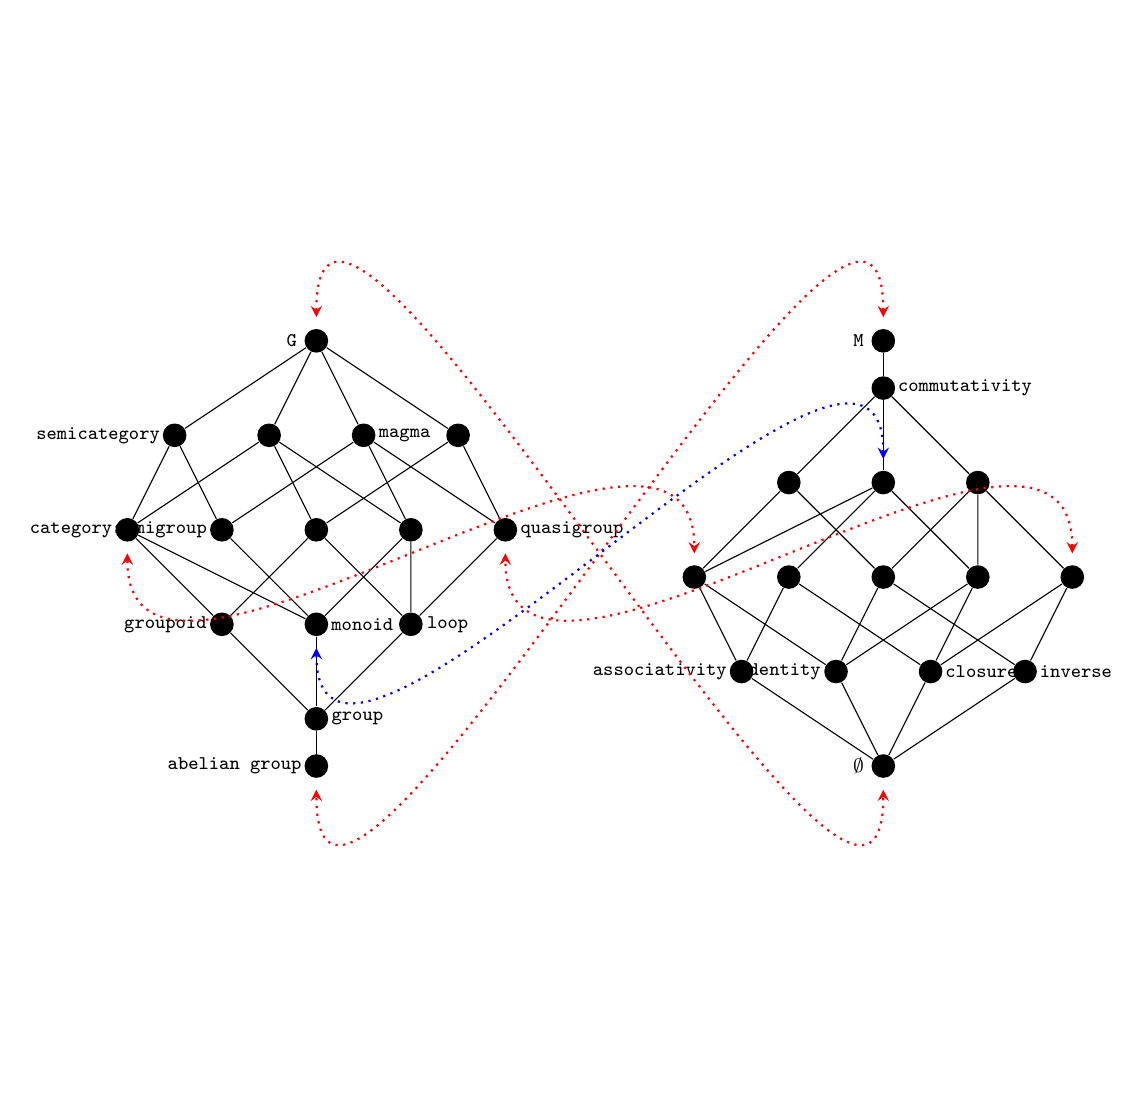
\begin{tikzpicture}[scale=0.6, every node/.style={circle, fill=black, inner sep=0.5pt, minimum size=3mm}]
    \node (a1) at (0,4) [label=left:{\scriptsize \texttt{G}}] {};

    \node (b1) at (-3,2) [label=left:{\scriptsize \texttt{semicategory}}] {};
    \draw (a1) -- (b1);

    \node (b2) at (-1,2) [label=left:{\scriptsize \texttt{}}] {};
    \draw (a1) -- (b2);

    \node (b3) at (1,2) [label=right:{\scriptsize \texttt{magma}}] {};
    \draw (a1) -- (b3);

    \node (b4) at (3,2) [label=right:{\scriptsize \texttt{}}] {};
    \draw (a1) -- (b4);

    \node (c1) at (-4,0) [label=left:{\scriptsize \texttt{category}}] {};
    \draw (c1) -- (b1);
    \draw (c1) -- (b2);

    \node (c2) at (-2,0) [label=left:{\scriptsize \texttt{semigroup}}] {};
    \draw (c2) -- (b1);
    \draw (c2) -- (b3);

    \node (c3) at (0,0) [label=left:{\scriptsize \texttt{}}] {};
    \draw (c3) -- (b2);
    \draw (c3) -- (b4);

    \node (c4) at (2,0) [label=right:{\scriptsize \texttt{}}] {};
    \draw (c4) -- (b2);
    \draw (c4) -- (b3);

    \node (c5) at (4,0) [label=right:{\scriptsize \texttt{quasigroup}}] {};
    \draw (c5) -- (b3);
    \draw (c5) -- (b4);

    \node (d1) at (-2,-2) [label=left:{\scriptsize \texttt{groupoid}}] {};
    \draw (d1) -- (c1);
    \draw (d1) -- (c3);

    \node (d2) at (0,-2) [label=right:{\scriptsize \texttt{monoid}}] {};
    \draw (d2) -- (c1);
    \draw (d2) -- (c2);
    \draw (d2) -- (c4);

    \node (d3) at (2,-2) [label=right:{\scriptsize \texttt{loop}}] {};
    \draw (d3) -- (c3);
    \draw (d3) -- (c4);
    \draw (d3) -- (c5);

    \node (e1) at (0,-4) [label=right:{\scriptsize \texttt{group}}] {};
    \draw (e1) -- (d1);
    \draw (e1) -- (d2);
    \draw (e1) -- (d3);

    \node (f1) at (0,-5) [label=left:{\scriptsize \texttt{abelian group}}] {};
    \draw (f1) -- (e1);

    \begin{scope}[shift={(12,0)}]
      \node (ra1) at (0,-5) [label=left:{\scriptsize $\emptyset$}] {};

      \node (rb1) at (-3,-3) [label=left:{\scriptsize \texttt{associativity}}] {};
      \draw (ra1) -- (rb1);

      \node (rb2) at (-1,-3) [label=left:{\scriptsize \texttt{identity}}] {};
      \draw (ra1) -- (rb2);

      \node (rb3) at (1,-3) [label=right:{\scriptsize \texttt{closure}}] {};
      \draw (ra1) -- (rb3);

      \node (rb4) at (3,-3) [label=right:{\scriptsize \texttt{inverse}}] {};
      \draw (ra1) -- (rb4);

      \node (rc1) at (-4,-1) [label=left:{\scriptsize \texttt{}}] {};
      \draw (rc1) -- (rb1);
      \draw (rc1) -- (rb2);

      \node (rc2) at (-2,-1) [label=left:{\scriptsize \texttt{}}] {};
      \draw (rc2) -- (rb1);
      \draw (rc2) -- (rb3);

      \node (rc3) at (0,-1) [label=left:{\scriptsize \texttt{}}] {};
      \draw (rc3) -- (rb2);
      \draw (rc3) -- (rb4);

      \node (rc4) at (2,-1) [label=right:{\scriptsize \texttt{}}] {};
      \draw (rc4) -- (rb2);
      \draw (rc4) -- (rb3);

      \node (rc5) at (4,-1) [label=right:{\scriptsize \texttt{}}] {};
      \draw (rc5) -- (rb3);
      \draw (rc5) -- (rb4);

      \node (rd1) at (-2,1) [label=left:{\scriptsize \texttt{}}] {};
      \draw (rd1) -- (rc1);
      \draw (rd1) -- (rc3);

      \node (rd2) at (0,1) [label=right:{\scriptsize \texttt{}}] {};
      \draw (rd2) -- (rc1);
      \draw (rd2) -- (rc2);
      \draw (rd2) -- (rc4);

      \node (rd3) at (2,1) [label=right:{\scriptsize \texttt{}}] {};
      \draw (rd3) -- (rc3);
      \draw (rd3) -- (rc4);
      \draw (rd3) -- (rc5);

      \node (re1) at (0,3) [label=right:{\scriptsize \texttt{commutativity}}] {};
      \draw (re1) -- (rd1);
      \draw (re1) -- (rd2);
      \draw (re1) -- (rd3);

      \node (rf1) at (0,4) [label=left:{\scriptsize \texttt{M}}] {};
      \draw (rf1) -- (re1);
    \end{scope}
    \draw[red, dotted, stealth-stealth, line width=0.8pt] (12,4.5) to[out=90, in=270] (0,-5.5);
    \draw[red, dotted, stealth-stealth, line width=0.8pt] (16,-0.5) to[out=90, in=270] (4,-0.5);
    \draw[red, dotted, stealth-stealth, line width=0.8pt] (-4,-0.5) to[out=270, in=90] (8,-0.5);
    \draw[red, dotted, stealth-stealth, line width=0.8pt] (0,4.5) to[out=90, in=270] (12,-5.5);
    \draw[blue, dotted, stealth-stealth, line width=0.8pt] (0,-2.5) to[out=270, in=90] (12,1.5);
  \end{tikzpicture}
  \vspace{-6em}
  \caption{The lattices induced by the closure systems $\mathcal{G}$ and $\mathcal{M}$. \textcolor{red}{Each node in a lattice represents
  the set comrpising of all labels reachable from below}}
  \label{figure:two-lattices}
\end{figure}

Earlier, it was suggested that Galois connections are particularly interesting when the closure systems they induce are themselves
interesting, and, future discussion of an example of such interesting closure systems was promised. Let us now give such an example, and in
doing so provide some intution for why Galois connections are a useful way of modelling concepts, to be introduced immediately afterwards.

Consider the concept derived from the algebraic structure of a \textit{monoid}: a set equipped with a binary operation that satisfies the properties
of closure, associativity, and that has an identity element. We should want to include in the extension of this concept all those algebraic
structures that would be considered subclasses of monoids. These are those structures which satisfy the properties of a monoid (and possibly
additional properties). Of course, a \textit{monoid} should be a member of this extension, since the condition by which structures are included
in the extension of this concept is that they satisfy closure, associativity, and have an identity element. Another structure we should
expect to see in this extension is a \textit{group}, which satisfies these requirements while also having the property of invertibility.

Now let us consider the concept derived from a \textit{group}. We have just shown that a group is a subclass of monoid, so it should follow that
the extension of a group must be a subset of the extension of a monoid. What of the intension? Suppose the intension of the concept of a monoid
were not a subset of that of a group, then monoids would have to satisfy some property that groups did not. This creates a contradiction, as
it would mean we could not properly consider a group to be a subclass of a monoid.

This reveals the relationship between concepts, such that when we move from the more general concept (monoid) to the more specific concept (group),
the extension becomes smaller while the intension grows. The extension of group is contained within the extension of monoid, but the
intension of monoid is contained within the intension of group. This contravariance between the extensions and intensions of concepts suggests
a clear hierarchical structure; moreoever, it is precisely described by Galois connections.

With this in mind, it is finally an appropriate time to define what is meant by \textit{formal concept}:

\begin{definition}
  \index{formal concept} \index{lattice! concept lattice} \label{definition:formal-concept} A \emph{formal concept} of a context $\GMI$ is a
  pair $(A,B)$ where $A \subseteq G$ and $B\subseteq M$ where $A^{\uparrow}= B$ and $B^{\downarrow}= A$. We call $A$ the \emph{concept
  extent} and $B$ the \emph{concept intent}. We write $\BGMI$ to denote the set of all concepts of $\GMI$.
\end{definition}

A concept is then a pair of closed sets, where each set represents either the extensional or intensional perspective on the concept. Indeed,
the extension and intension are related by virtue of being the inverses of one another under the derivation operators, and so there is a
degree of redundancy in this definition since knowing the concept extension is sufficient to learning the concept intension and vice verse
\cite{ganter2016conceptual}. Yet, we persevere with this redundancy as it offers a unifying perspective.

One pleasing consequence of the definition of a formal concept is that, for any set $A\subseteq G$ of objects, the set $A^{\uparrow}$ will
always be a concept intent, and facilitates the construction of $(A^{\uparrow \downarrow}, A^{\uparrow})$ which is similarly always a concept;
in general, the set $A$ is a concept extent if it is equal to its' closure $A^{\uparrow \downarrow}$. The dual perspective holds, and so for
a set $B \subseteq M$ of attributes, $B^{\downarrow}$ is always a concept extent. We are even more fortunate in that we have already
extensively discussed the collection(s) of closed sets of objects and attributes and what structure they might have: of course, these are the
closure systems $\mathcal{G}$ and $\mathcal{M}$ and their corresponding lattice structure.

To make this idea concrete, we reconsider the previous discussion where we (informally) described the concept of a monoid. It follows that the
derivation $\{\texttt{monoid }\}^{\uparrow}$ yields the intent $\{\texttt{closure,associativity,identity}\}$. In turn, the derivation of the
concept intent results in the set $\{\texttt{monoid,group,abelian group}\}$, which is the concept extent, and so
\[
  \big(\{\texttt{monoid,group,abelian group}\}, \{\texttt{closure,associativity,identity }\}\big)
\]
is a formal concept of \Cref{cxt:grouplikes}.

The union of concept extents (intents) is not guaranteed to yield another concept extent (intent), whereas the intersection of concept
extents (intents) will always result in another concept extent (intent). That is to say, the closure systems $\mathcal{G}$ and $\mathcal{M}$
are not closed under taking arbitrary unions, while they are under arbitrary intersections.

\begin{proposition}
  \label{proposition:intersection-union-concepts} Let $T$ be an indexing set, then for every $t \in T$ $A_{t}\subseteq G$ is a set of
  objects, then
  \[
    \big( \underset{t \in T}\bigcup A_{t}\big)^{\uparrow}= \underset{t \in T}\bigcap A_{t}^{\uparrow}
  \]
\end{proposition}

If we examine the lattices in \Cref{figure:two-lattices}, we observe that the two derivation operators map to and from the concept intent and
extent (shown by the dotted blue arrows). This observation suggests a more consolidated perspective: The two lattices can be unified into a single
structure where elements of the lattice are precisely the pairs $(A,B)$ where $A \in \mathcal{G}$ and $B \in \mathcal{M}$ and also $A^{\uparrow}
= B$ and $B^{\downarrow}= A$. In other words, the lattice of concepts. We appropriately call this structure the \textit{concept lattice} of a
formal context, and write $\CLGMI$ to refer to the set of all concepts equipped with this structure.

\begin{figure}[H]
  \centering
  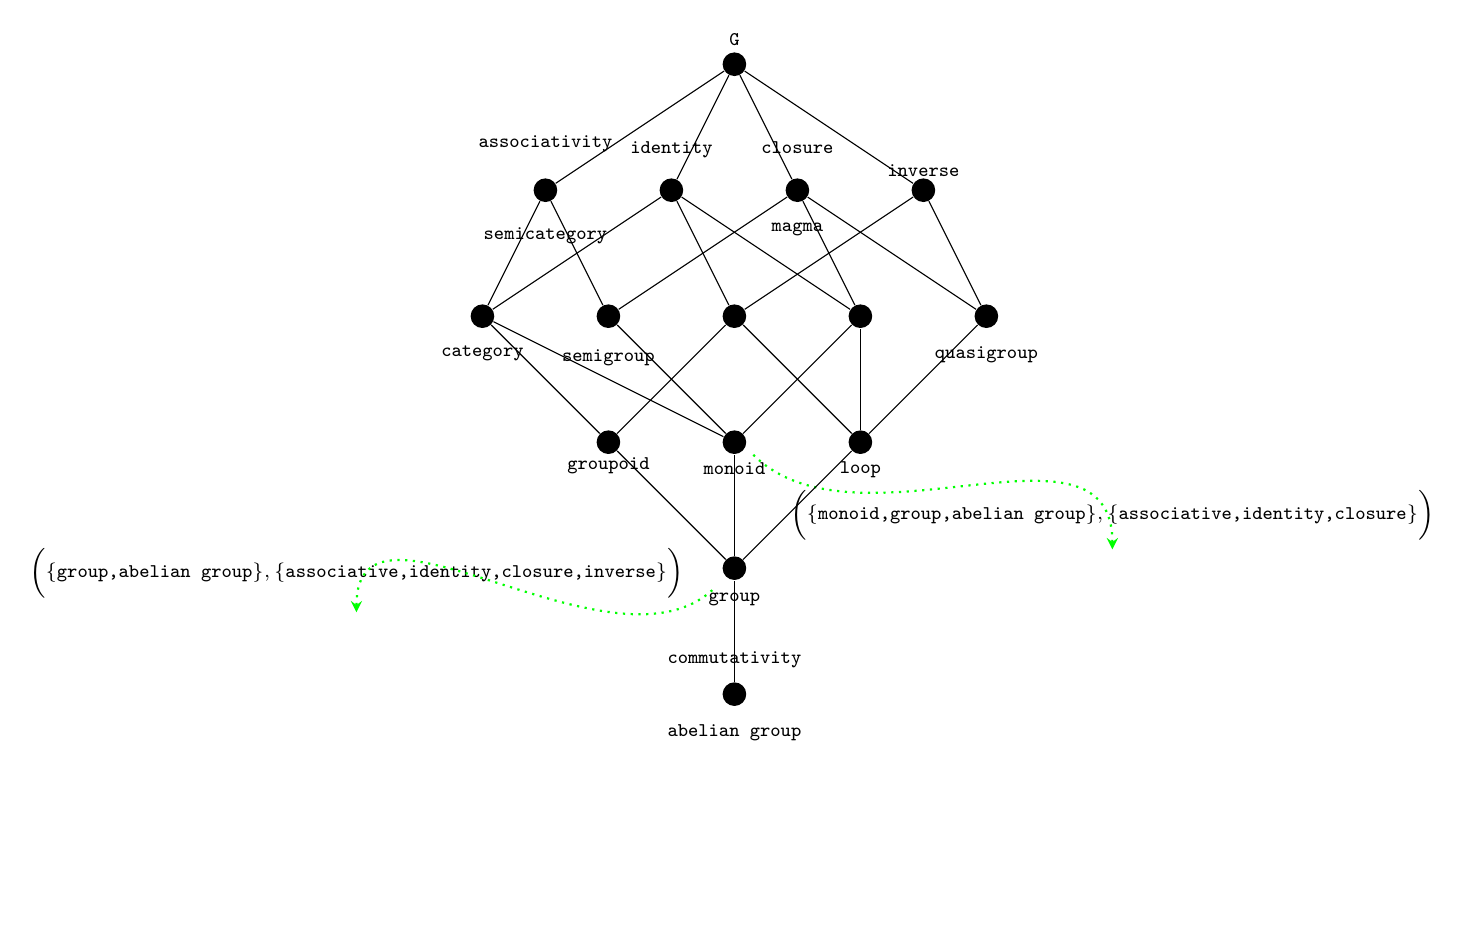
\begin{tikzpicture}[scale=0.8, every node/.style={circle,fill=black,inner sep=0.5pt,minimum size=3mm}]
    %––––– row 1 –––––
    \node (a1) at (0,4) [label={[anchor=south,yshift=0mm]above:{\scriptsize\texttt{G}}}] {};

    %––––– row 2 –––––
    \node (b1)
      at
      (-3,2)
      [
        label={[anchor=south,yshift=-4.5mm]above:{\scriptsize\texttt{associativity}}},
        label={[anchor=north,yshift=4.5mm,text depth=0pt]below:{\scriptsize\strut\texttt{semicategory}}}
      ]
      {};
    \draw (a1) -- (b1);

    \node (b2) at (-1,2) [label={[anchor=south,yshift=-2mm]above:{\scriptsize\texttt{identity}}}] {};
    \draw (a1) -- (b2);

    \node (b3)
      at
      (1,2)
      [
        label={[anchor=south,yshift=-1mm]above:{\scriptsize\texttt{closure}}},
        label={[anchor=north,yshift=1mm,text depth=0pt]below:{\scriptsize\strut\texttt{magma}}}
      ]
      {};
    \draw (a1) -- (b3);

    \node[fill=none]
      (eg)
      at
      (6,-8)
      [
        label={[anchor=south,yshift=-4mm]above:{\scriptsize $\big(\{\texttt{monoid,group,abelian group}\},\{\texttt{associative,identity,closure}\}\big)$ }}
      ]
      {};
    \draw[green, dotted, stealth-, line width=0.8pt] (6,-3.7) to[out=90, in=315] (0.3,-2.2);

    \node[fill=none]
      (eg1)
      at
      (-6,-9)
      [
        label={[anchor=south,yshift=-4mm]above:{\scriptsize $\big(\{\texttt{group,abelian group}\},\{\texttt{associative,identity,closure,inverse}\}\big)$ }}
      ]
      {};
    \draw[green, dotted, stealth-, line width=0.8pt] (-6,-4.7) to[out=90, in=225] (-0.3,-4.3);

    \node (b4) at (3,2) [label={[anchor=south,yshift=-4mm]above:{\scriptsize\texttt{inverse}}}] {};
    \draw (a1) -- (b4);

    \node (c1) at (-4,0) [label={[anchor=north,yshift=3mm,text depth=0pt]below:{\scriptsize\strut\texttt{category}}}] {};
    \draw (c1) -- (b1);
    \draw (c1) -- (b2);

    \node (c2) at (-2,0) [label={[anchor=north,yshift=3mm,text depth=0pt]below:{\scriptsize\strut\texttt{semigroup}}}] {};
    \draw (c2) -- (b1);
    \draw (c2) -- (b3);

    \node (c3) at (0,0) {};
    \draw (c3) -- (b2);
    \draw (c3) -- (b4);

    \node (c4) at (2,0) {};
    \draw (c4) -- (b2);
    \draw (c4) -- (b3);

    \node (c5) at (4,0) [label={[anchor=north,yshift=4mm,text depth=0pt]below:{\scriptsize\strut\texttt{quasigroup}}}] {};
    \draw (c5) -- (b3);
    \draw (c5) -- (b4);

    \node (d1) at (-2,-2) [label={[anchor=south,yshift=-7mm]below:{\scriptsize\texttt{groupoid}}}] {};
    \draw (d1) -- (c1);
    \draw (d1) -- (c3);

    \node (d2) at (0,-2) [label={[anchor=south,yshift=-6mm]below:{\scriptsize\texttt{monoid}}}] {};
    \draw (d2) -- (c1);
    \draw (d2) -- (c2);
    \draw (d2) -- (c4);

    \node (d3) at (2,-2) [label={[anchor=south,yshift=-5mm]below:{\scriptsize\texttt{loop}}}] {};
    \draw (d3) -- (c3);
    \draw (d3) -- (c4);
    \draw (d3) -- (c5);

    \node (e1) at (0,-4) [label={[anchor=south,yshift=-6mm]below:{\scriptsize\texttt{group}}}] {};
    \draw (e1) -- (d1);
    \draw (e1) -- (d2);
    \draw (e1) -- (d3);

    \node (f1)
      at
      (0,-6)
      [
        label={[anchor=south,yshift=-6mm]above:{\scriptsize\texttt{commutativity}}},
        label={[anchor=north,yshift=6mm,text depth=0pt]below:{\scriptsize\strut\texttt{abelian group}}}
      ]
      {};
    \draw (f1) -- (e1);
  \end{tikzpicture}
  \caption{The concept lattice corresponding to \Cref{cxt:grouplikes}}
  \label{figure:concept-lattice-group-likes}
\end{figure}

\begin{remark}
  Reading a concept lattice requires a small amount of getting used to: The labels above a node in the diagram correspond to attributes, while
  objects are labelled below a node. Each node represents a concept $C \in \BGMI$. The extension of $C$ contains all objects attached to nodes
  which have a (strictly) downwards path from $C$, while the intension of $C$ contains those attributes labelled at nodes where there is a
  strictly upwards path from $C$.
\end{remark}

The concept lattice is isomorphic to the closure system $\mathcal{G}$ of objects, and dually isomorphic to the closure system $\mathcal{M}$ of
attributes. We now consider the first part of the fundamental result in FCA.

\begin{theorem}[The Basic Theorem of Concept Lattices: Part one]
  \label{theorem:basic-theorem-part1} The concept lattice $\CLGMI$ of a formal context is a complete lattice in which meets and joins are given
  by
  \begin{align*}
     & \underset{t \in T}\bigwedge (A_{t}, B_{t}) = \Big( \underset{t \in T}\bigcap A_{t}, \; \big(\underset{t \in T}\bigcup B_{t}\big)^{\downarrow \uparrow}\Big) \\
     & \underset{t \in T}\bigvee (A_{t}, B_{t}) = \Big( \big(\underset{t \in T}\bigcup A_{t}\big)^{\uparrow \downarrow},\; \underset{t \in T}\bigcap B_{t}\Big)
  \end{align*}
\end{theorem}

Part one of the basic theorem describes how we might find the meet and join of concepts in the concept lattice. To make this clear, recall the
isomorphism between $\mathcal{G}$ and $\CLGMI$, which tells us that
\[
  A_{0}\wedge A_{1}\cong (A_{0},B_{0}) \wedge (A_{1},B_{1})
\]
for any $A_{0},A_{1}\in \mathcal{G}$ where $(A_{i},B_{i})$ is the concept with extent $A_{i}$.

The isomorphism between the concept lattice $\CLGMI$ and the lattice corresponding to the closure system $\mathcal{G}$ means that the meet
of any two concepts can be found by considering the concept formed by the meet of their extensions with respect to $\mathcal{G}$. Of course,
since $\mathcal{G}$ is a closure system, the meet operation on this lattice corresponds to taking the intersection of these extensions (and
$\mathcal{G}$ is closed under arbitrary intersections). As there is a dual isomorphism between $\CLGMI$ and $\mathcal{M}$, we can equivalently
discover the meet of two concepts by considering the join operation on the concept intensions with respect to the lattice of $\mathcal{M}$.
This corresponds to taking the closure of the union of concept intensions (cf. \Cref{theorem:closure-systems-lattices} for a reminder of why).

The join of two concepts---again, due to the dual isomorphism---corresponds to the meet operation on the concept extensions with respect to
the lattice of $\mathcal{M}$ and can thus be found by taking the intersection of their intensions, under which $\mathcal{M}$ is closed. Or, by
the join operation on $\mathcal{G}$, which corresponds to the closure of the union of extensions.

For another perspective, consider that each $A_{t}$ is equivalent to $B_{t}^{\downarrow}$. By \Cref{proposition:intersection-union-concepts}
\begin{align*}
   & \underset{t \in T}\bigwedge (A_{t}, B_{t}) = \Big( \underset{t \in T}\bigcap A_{t}, \; \big(\underset{t \in T}\bigcup B_{t}\big)^{\downarrow \uparrow}\Big)
\end{align*}
can be restated as
\begin{align*}
   & \underset{t \in T}\bigwedge (A_{t}, B_{t}) = \Big(\big(\underset{t \in T}\bigcup B_{t}\big)^{\downarrow}, \; \big(\underset{t \in T}\bigcup B_{t}\big)^{\downarrow \uparrow}\Big)
\end{align*}
We may arrive at the concept lattice in another way, by considering the rather natural order on concepts which arises from the \textit{subconcept--superconcept}
relation. We had, earlier, discussed that `group' is a subclass of `monoid', and so the extension of the associated concept of a group
should be a subset of that of a monoid. In line with this, we say that a concept $(A_{0},B_{0})$ is a subconcept of another $(A_{1},B_{1})$
if and only if $A_{0}\subseteq A_{1}$. Dually, $(A_{1},B_{1})$ is a superconcept of $(A_{0},B_{0})$ if and only if $B_{1}\subseteq B_{0}$. In
this case we write $(A_{0},B_{0}) \leq (A_{1},B_{1})$. When considering the set of concepts $\BGMI$ with the relation defined by $\leq$, the
resulting structure is the same concept lattice $\CLGMI$ from before. As an illustration, consider the two selected concepts in \Cref{figure:concept-lattice-group-likes}.

% \subsection{Weaker Concepts}
% \label{subsection:weaker-concepts} \textcolor{red}{I was going to introduce existing ideas in FCA about ``protoconcepts''; but I think maybe
% this should be done right before we discuss typical concepts. }

\section{Contextual Attribute Logic}
\label{section:contextual-attribute-logic}

In addition to the set of attributes $M$ of a formal context, consideration can be expanded to the idea of \textit{compound attributes}. The
additional expressivity enabled by compound attributes is akin to that which formulae give to propositional atoms. Compound attributes are constructed
by defining rules for combinations of ``normal'' attributes, in almost complete analogy to propositional atoms constructing formulae under
the Boolean connectives.

There is, however, a meaningful distinction between the perspectives that one should adopt when considering either attribute or
propositional logic. Where propositional atoms and their constructed formulae are viewed in terms of truth, it is more helpful to consider
compound attributes as descriptors of objects \cite{ganter2024formal,ganter2025language}. With this perspective in mind, we introduce
compound attributes inductively as:

\begin{definition}
  \label{definition:compound-attributes}

  Let $M$ be a set of attributes (as we might find in a formal context). The set $\mathcal{M}$ of \emph{compound attributes} over $M$ is
  defined by
  \begin{itemize}
    \item Every attribute $m \in M$ is a compound attribute \hfill ($M \subseteq \mathcal{M}$)

    \item If $\varphi \in \mathcal{M}$ is a compound attribute, then so is $\neg \varphi$ \hfill ($\neg \varphi \in \mathcal{M}$)

    \item If $\Gamma \subseteq \mathcal{M}$ is a set of compound attributes, then $\bigwedge \Gamma$ is a compound attribute \hfill ($\bigwedge
      \Gamma \in \mathcal{M}$)
  \end{itemize}
\end{definition}

We distinguish between compound and ``normal'' attributes by using lowercase Greek letters for compound attributes, and lowercase Latin
letters for attributes. The semantics of compound attributes are defined relative to a given formal context, and the respective derivation
operators, and so we have:

\begin{definition}
  \label{definition:compound-attributes-semantics}

  In a formal context $\GMI$ the extension of each compound attribute $\varphi \in \mathcal{M}$ is written $\varphi^{\Vdash}$ and defined as
  \begin{itemize}
    \item If $\varphi$ is a ``plain'' attribute (i.e., $\varphi \in M$) then $\varphi^{\Vdash}\coloneq \varphi^{\downarrow}$

    \item If $\varphi$ is the negation of another compound attribute $\gamma \in \mathcal{M}$ then $\varphi^{\Vdash}\coloneq G \setminus \gamma
      ^{\Vdash}$

    \item If $\varphi$ is the result of a conjunction of a set of compound attributes $\bigwedge \Gamma$ then $\varphi^{\Vdash}\coloneq \underset
      {\gamma \in \Gamma}\bigcap \gamma^{\Vdash}$
  \end{itemize}
  For an object $g\in G$ and compound attribute $\varphi \in \mathcal{M}$ we write $g \Vdash \varphi$ if and only if
  $g \in \varphi^{\Vdash}$, and say that $g$ \say{satisfies} $\varphi$.
\end{definition}

It is clear that this definition allows for the construction of an infinite number of compound attributes, which is unhelpful. Things can be
made simpler with the introduction of \textit{extensional} and \textit{global equivalence}. Two compound attributes $\varphi, \gamma \in \mathcal{M}$
are extensionally equivalent with respect to a context $\GMI$ if their extensions are the same. If $\varphi^{\Vdash}= \gamma^{\Vdash}$. There
is a global equivalence between $\varphi$ and $\gamma$ if they are extensionally equivalent in any possible context with the attribute set $M$.

Disjunction may appear to be missing from this definition, but this is merely a syntactic omission. The construction of a compound attribute
of the form $\bigvee \Gamma$ with the extension $\underset{\gamma \in \Gamma}\bigcup \gamma^{\Vdash}$ is equivalent to $\neg \underset{\gamma \in \Gamma}
\bigwedge \neg \gamma$.

In propositional logic, we might construct a formula by taking the conjunction operation over a set of formulae. It is, however, a requirement
that this set be finite. Compound attributes do not have this requirement, and so when we write $\bigwedge \Gamma$, it is perfectly possible
for $\Gamma$ to be infinite. Later on in \Cref{chapter:defeasible-reasoning-in-fca}, we rely on this finiteness property holding in compound
attributes, and so we offer a new inductive definition. In future, when we speak about compound attributes it can be assumed that we mean compound
attributes as per this second definition.

\begin{definition}
  \label{definition:compound-attributes-2} Let $M$ be a set of attributes, then the language of (finite) compound attributes is inductively
  as
  \begin{align}
    \phi ::= m \mid (\neg \phi) \mid (\phi_{1}\lor \phi_{2}) \mid (\phi_{1}\land \phi_{2}) \mid (\phi_{1}\rightarrow \phi_{2})
  \end{align}
  where $m \in M$ is a ``plain'' attribute. Then, the satisfaction relation $\Vdash$ is

  \begin{itemize}
    \item $g \Vdash \varphi$ if and only if $g \in \varphi^{\downarrow}$

    \item $g \Vdash \neg \varphi$ if and only if $g \in G \setminus \varphi^{\Vdash}$

    \item $g \Vdash \varphi \lor \gamma$ if and only if $g \in \varphi^{\Vdash}\cup \gamma^{\Vdash}$

    \item $g \Vdash \varphi \land \gamma$ if and only if $g \in \varphi^{\Vdash}\cap \gamma^{\Vdash}$

    \item $g \Vdash \varphi \rightarrow \gamma$ if and only if $g \in \neg \varphi^{\Vdash}\lor \gamma^{\Vdash}$
  \end{itemize}
\end{definition}

\begin{example}
  Consider the context below, which represents a portion of the $1984$ United States Congressional voting records taken from the UC Irvine
  Machine Learning repository \cite{congressional_voting_records_105}.

  \begin{figure}[H]
    \centering
    \begin{cxt}
      \label{cxt:voting} \cxtName{\textbf{\texttt{Congressional Voting Records}}} \atr{\texttt{mx-missile}} \atr{\texttt{crime}} \atr{\texttt{immigration}}
      \atr{\texttt{satellite ban}} \atr{\texttt{education}} \atr{\texttt{republican}} \atr{\texttt{democrat}} \obj{.xx.xx.}{\texttt{Representative 1}}
      \obj{......x}{\texttt{Representative 4}} \obj{.x..xx.}{\texttt{Representative 9}} \obj{..x.x.x}{\texttt{Representative 17}}
    \end{cxt}
    \caption{A context describing a portion of congressional voting records for 1984}
    \label{figure:voting-records}
  \end{figure}

  We can construct meaningful compound attributes such as $\texttt{education}\land \neg \texttt{immigration}$, the extension of which
  consists of all representatives who voted ``yay'' with respect to the education bill, and either abstained or voted ``nay'' to the immigration
  bill. This compound attribute is extensionally equivalent to $\texttt{republican}\land \neg \texttt{immigration}$.

  We may be tempted to say that $\texttt{republican}$ and $\neg \texttt{democrat}$ are globally equivalent compound attributes; but this would
  be an error. Globally equivalent attributes have the same extension in any conceivable context, not only those which align with background
  assumptions about the nature of the attributes. For an example of global equivalence, consider $\texttt{democrat}$ and $\neg \neg \texttt{democrat
  }$.
\end{example}

In general, to determine if two compound attributes $\varphi$ and $\psi$ are globally equivalent we need only consider a single context
which has an object for each combination of normal attributes. We call such a context the \textit{test context}, and write $(\pset{M},M,\in)$.

\section{Attribute Implications}
\label{section:attribute-implications}Attribute implications in FCA are a way of representing dependencies that exist between (sets of)
attri butes in a context.
\begin{definition}
  \label{definition:attribute-implication} Let $M$ be a non-empty set of attributes, then an \emph{attribute implication} is an expression of
  the form
  \[
    A \rightarrow B
  \]
  where $A,B \subseteq M$. We call $A$ the \emph{antecedent} and $B$ the \emph{consequent} of the implication.
\end{definition}
The semantics of attribute implications will be familiar to anyone who has seen material implications, and so
\begin{definition}
  \label{definition:attribute-implication-semantics} Let $M$ be a non-empty set of attributes, and $A,B,C \subseteq M$ three subsets. Then we
  say that $C$ \emph{respects} the implication $A \rightarrow B$ if and only if $B \subseteq C$ or $A \not \subseteq C$, and we write $C \vDash
  A \rightarrow B$.
\end{definition}
Considering the context in \Cref{figure:voting-records}, an example of an attribute implication is$\texttt{crime}\rightarrow \texttt{immigration
}$. If we examine the context in \Cref{figure:voting-records}it is apparent that every representative who voted in favour of the proposed c
rime bill also voted in favour of the immigration bill; we write this dependency as$\texttt{crime }\rightarrow \texttt{immigration }$.

When discussing implications between singleton sets of attributes, we may choose to omit the brackets and write$A \rightarrow m$in lieu of$A
\rightarrow \{m\}$.

% \begin{lemma}
%   \label{lemma:surjective-operators} Let $\GMI$ be a context with $(\uparrow, \downarrow)$ as the usual derivation operators. The closure systems
%   \[
%     \mathcal{G}\;=\; \{\,A\subseteq G \mid A^{\uparrow\downarrow}=A\,\}, \qquad \mathcal{M}\;=\; \{\,B\subseteq M \mid B^{\downarrow\uparrow}=B\,\}
%   \]
%   Then
%   \[
%     \mathcal{M}\;=\; \{\,A^{\uparrow}\mid A\subseteq G\,\}, \qquad \mathcal{G}\;=\; \{\,B^{\downarrow}\mid B\subseteq M\,\},
%   \]
%   and so $(\cdot)^{\uparrow}$ and $(\cdot)^{\downarrow}$ are surjective onto $\mathcal{M}$ and $\mathcal{G}$, respectively.
% \end{lemma}

% \begin{proof}
%   \label{proof:surjective-operators} We prove the statement for $(\cdot)^{\uparrow}$; the dual argument follows by swapping $G$ with $M$ and $\uparrow$ with $\downarrow$. Let $B \in \mathcal{M}$, then
%   by definition $B = B^{\downarrow \uparrow}$. Let some $A \subseteq G$ so that $A = B^{\downarrow}$.
% \end{proof}

% % To make formal the earlier example, $\big(\{\texttt{monoid,group,abelian group}\}, \{\texttt{closure,associativity,identity}\} \big)$ is a concept of the context in \Cref{cxt:grouplikes}.
% \textcolor{red}{I want to say something about how each operator is a map onto the closure system for its codomain. The next paragraph follows from this remark}

% From the Galois connection, for every subset $A\subseteq G$ of objects, the derivation $A^{\uparrow}$ of the subset is precisely a concept intent, and so $(A^{\uparrow \downarrow}, A^{\uparrow})$ always
% describes a concept. If this is not immediately obvious, consider that the derivation operator $(\cdot)^{\uparrow}\colon \pset{G}\to \pset{M}$ is onto the closure system $\mathcal{M}$, and can be
% described by
% %
% \begin{align*}
%   A^{\uparrow}= \bigcap \; \{g^{\uparrow}\mid g \in A \}
% \end{align*}

% Each object $g \in A$ is mapped to its object intent $g^{\uparrow}$ for which $g^{\uparrow}\in \mathcal{M}$, since $\mathcal{M}$ is closed under arbitrary intersections it follows that
% $A^{\uparrow}\in \mathcal{M}$, and so $A^{\uparrow}$ is closed.

% \clearpage
% Since $(\uparrow, \downarrow)$ constitute a Galois connection on the powersets $\pset{G}$ and $\pset{M}$, we can find two closure systems on $G$ and $M$, respectively.

% From \Cref{proposition:derivation-operators-galois} we can describe two closure operators $(\cdot)^{\uparrow \downarrow}$ and $(\cdot)^{\downarrow \uparrow}$ on the powersets $\pset{G}$ and $\pset{M}$,
% respectively.

% And so, $A^{\uparrow \downarrow}$---which can rather cumbersomely be described as \say{The set of all objects which satisfy all the attributes satisfied by \texttt{semigroup} and \texttt{monoid}}---would
% yield the set $\{\texttt{semigroup, monoid, group, abelian group}\}$. In fact, this composition of derivation operators satisfies very specific properties.%

% With the above relationship between sets of objects and attributes in mind, it is appropriate to introduce a \textit{formal concept}.

% It is no coincidence, as we will see later on, that this corresponds to taking the intersection of each object's intent, and so we have equivalently for a set of objects $A \subseteq G$

% \begin{align*}
%   A^{\uparrow}= \bigcap \{g^{\uparrow}\mid g \in A \} \quad \textit{(resp.)}\quad B^{\downarrow}= \bigcap \{m^{\downarrow}\mid m \in B\}
% \end{align*}

% \begin{example}
%   \label{example:formal-concept} If we consider the \texttt{groupoid} object from \Cref{cxt:grouplikes}, we can derive the concept:

%   \[
%     \big(\{\texttt{groupoid,group,abelian group}\}, \{\texttt{associativity,identity,closure }\} \big)
%   \]

%   % The derivation of \texttt{groupoid} yields $\{\texttt{associativity,identity,closure}\}$, by \Cref{equation:galois-3} this set is closed under its Galois connection, and formsc a concept intent.

%   % To begin, the object intent $\texttt{groupoid}^\uparrow$ is determined, which yields the set $\{\texttt{associativity,identity,closure}\}$. From \Cref{proposition:properties-about-derivation-operators} this set is closed, and represents a concept intent. The concept extent is determined by application of a derivation operator to the concept intent.
% \end{example}

% The set of all concepts has a natural ordering induced on it by the \textit{subconcept--superconcept} relation. If $(A_{0},B_{0})$ and $(A_{1},B_{1})$ are two concepts, then $(A_{0},B_{0})$ is a
% \textit{subconcept} of $(A_{1}, B_{1})$ and $(A_{1}, B_{1})$ is a superconcept of $(A_{0},B_{0})$ if and only if $A_{0}\subseteq A_{1}$. Equivalently if $B_{1}\subseteq B_{0}$. We denote set of all concepts
% ordered in this way by $\CLGMI$, and call this set the \textit{concept lattice} of $\GMI$.

% Intuitively, one concept is a subconcept of another, if every instance of the first concept is also an instance of the second. From the Galois connection, this is equivalently, albeit less intuitively,
% explained by every attribute of the second concept being included in the first.

% We can prescribe a rather intuitive ordering over concepts induced by the \textit{subconcept–superconcept} relation.
% \begin{figure}[H]
%   \centering
%   \begin{tikzpicture}[scale=0.8, every node/.style={circle, fill=black, inner sep=0.5pt,minimum size=0mm}]
%     \node (a1) at (0,3) [label=above:{\scriptsize $\top$}] {w};
%     % \node[draw=none, fill=none] at (0,3.5) {\tiny Top};

%     \node (b1) at (-3,1) [label=above:{\scriptsize \texttt{associativity}}] {};
%     \draw (a1) -- (b1);

%     \node (b2) at (-1,1) [label=above:{\scriptsize \texttt{identity}}] {z};
%     \draw (a1) -- (b2);

%     \node (b3) at (1,1) [label=above:{\scriptsize \texttt{closure}}, label=below:{\scriptsize \texttt{magma}}] {};
%     \draw (a1) -- (b3);

%     \node (b4) at (3,1) [label=above:{\scriptsize \texttt{inverse}}] {};
%     \draw (a1) -- (b4);

%     \node (c1) at (-4,-1) [label=below:{\scriptsize \texttt{category}}] {};
%     \draw (c1) -- (b1);
%     \draw (c1) -- (b2);

%     \node (c2) at (-2,-1) [label=below:{\scriptsize \texttt{semigroup}}] {};
%     \draw (c2) -- (b1);
%     \draw (c2) -- (b3);

%     \node (c3) at (0,-1) {};
%     \draw (c3) -- (b2);
%     \draw (c3) -- (b3);

%     \node (c4) at (2,-1) {};
%     \draw (c4) -- (b2);
%     \draw (c4) -- (b4);

%     \node (c5) at (4,-1) [label=below:{\scriptsize \texttt{quasigroup}}] {};
%     \draw (c5) -- (b3);
%     \draw (c5) -- (b4);

%     \node (d1) at (-2,-3) [label=below:{\scriptsize \texttt{monoid}}] {};
%     \draw (d1) -- (c1);
%     \draw (d1) -- (c2);
%     \draw (d1) -- (c3);

%     \node (d2) at (0,-3) [label=below:{\scriptsize \texttt{groupoid}}] {};
%     \draw (d2) -- (c1);
%     \draw (d2) -- (c3);

%     \node (d3) at (2,-3) [label=below:{\scriptsize \texttt{loop}}] {};
%     \draw (d3) -- (c3);
%     \draw (d3) -- (c4);
%     \draw (d3) -- (c5);

%     \node (e1) at (0,-5) [label=below:{\scriptsize \texttt{group}}] {};
%     \draw (e1) -- (d1);
%     \draw (e1) -- (d2);
%     \draw (e1) -- (d3);

%     \node (f1) at (0,-7) [label=above:{\scriptsize \texttt{commutativity}}, label=below:{\scriptsize \texttt{abelian group}}] {};
%     \draw (f1) -- (e1);
%   \end{tikzpicture}
%   \caption{The concept lattice associated with the formal context in \Cref{cxt:grouplikes}}
% \end{figure}

% \subsection{Attribute Implications}
% \label{subsection:attribute-implications}

% In FCA, attribute implications represent dependencies that exist between attributes in a context. If $M$ is a non-empty set of attributes with $A, B \subseteq M$, then we denote an attribute
% implication over $M$ as $A \rightarrow B$.

% \begin{definition}
%   \label{definition:attribute-implication} Let $M$ be a non-empty set of attributes, then an \emph{attribute implication} over $M$ is a
% \end{definition}

% If we examine the context in \Cref{context:voting-records-small} it is apparent that every representative who voted in favour of the proposed crime bill also voted in favour of the immigration bill;
% we write this dependency as $\texttt{crime }\rightarrow \texttt{immigration}$.

% \begin{figure}[H]
%   \centering
%   \begin{cxt}
%     \cxtName{\textbf{\texttt{Congressional Voting Records}}} \atr{\texttt{mx-missile}} \atr{\texttt{crime}} \atr{\texttt{immigration}} \atr{\texttt{satellite ban}} \atr{\texttt{education}} \atr{\texttt{republican}}
%     \atr{\texttt{democrat}} \obj{.xx.xx.}{\texttt{Representative 1}} \obj{......x}{\texttt{Representative 4}} \obj{.x..xx.}{\texttt{Representative 9}} \obj{..x.x.x}{\texttt{Representative 17}}
%   \end{cxt}
%   \caption{A context describing a portion of congressional voting records for 1984}
%   \label{context:voting-records-small}
% \end{figure}

% \clearpage

% \begin{figure}[H]
%   \centering
%   \small
%   \begin{cxt}
%     \label{cxt:people} \cxtName{\textbf{\texttt{Characters}}} \att{\texttt{human}} \att{\texttt{tralfamadorian}} \att{\texttt{linear time}} \att{\texttt{soldier}} \att{\texttt{optometrist}} \att{\texttt{pacifist}}
%     \obj{x..xxx}{\texttt{Billy Pilgrim}} \obj{x.xx..}{\texttt{Edgar Derby}} \obj{x....x}{\texttt{Montana Wildhack}} \obj{.x....}{\texttt{Zookeeper}}\obj{x.xx..}{\texttt{Paul Lazzaro}} \obj{x.x.x.}{\texttt{Lionel Merble}}
%     \obj{.x.x..}{\texttt{Test Pilot}}
%   \end{cxt}
%   \caption{A formal context showing necessary properties of group-like structures.}
% \end{figure}

% \begin{figure}[H]
%   \centering
%   \begin{tikzpicture}[scale=0.6, every node/.style={circle, fill=black, inner sep=0.5pt, minimum size=0mm}]
%     \node (a1) at (0,4) [label=left:{\scriptsize \texttt{G}}] {w};

%     \node (b1) at (-2,2) [label=left:{\scriptsize \texttt{}}] {};
%     \draw (a1) -- (b1);

%     \node (b2) at (0,2) [label=left:{\scriptsize \texttt{}}] {z};
%     \draw (a1) -- (b2);

%     \node (b3) at (2,2) [label=right:{\scriptsize \texttt{zookeeper}}] {};
%     \draw (a1) -- (b3);

%     \node (c1) at (-4,0) [label=left:{\scriptsize \texttt{montanna}}] {};
%     \draw (c1) -- (b1);

%     \node (c2) at (-2,0) [label=left:{\scriptsize \texttt{}}] {};
%     \draw (c2) -- (b1);
%     \draw (c2) -- (b2);

%     \node (c3) at (-0,0) [label=left:{\scriptsize \texttt{}}] {};
%     \draw (c3) -- (b1);

%     \node (c4) at (2,0) [label=right:{\scriptsize \texttt{}}] {};
%     \draw (c4) -- (b1);

%     \node (c5) at (4,0) [label=right:{\scriptsize \texttt{quasigroup}}] {};
%     \draw (c5) -- (b2);
%     \draw (c5) -- (b3);

%     \node (d1) at (-2,-2) [label=left:{\scriptsize \texttt{edgar,paul}}] {};
%     \draw (d1) -- (c2);
%     \draw (d1) -- (c4);

%     \node (d2) at (1,-2) [label=right:{\scriptsize \texttt{lionel}}] {};
%     \draw (d2) -- (c3);
%     \draw (d2) -- (c4);

%     \node (e1) at (-3,-4) [label=right:{\scriptsize \texttt{billy}}] {};
%     \draw (e1) -- (c1);
%     \draw (e1) -- (c2);
%     \draw (e1) -- (c3);

%     \node (f1) at (0,-5) [label=left:{\scriptsize $\emptyset$}] {};
%     \draw (f1) -- (e1);
%     \draw (f1) -- (d1);
%     \draw (f1) -- (d2);
%     \draw (f1) -- (c5);

%     \begin{scope}[shift={(12,0)}]
%       \node (ra1) at (0,-5) [label=left:{\scriptsize $\emptyset$}] {w};

%       \node (rb1) at (-3,-3) [label=left:{\scriptsize \texttt{associativity}}] {};
%       \draw (ra1) -- (rb1);

%       \node (rb2) at (-1,-3) [label=left:{\scriptsize \texttt{identity}}] {z};
%       \draw (ra1) -- (rb2);

%       \node (rb3) at (1,-3) [label=right:{\scriptsize \texttt{closure}}] {};
%       \draw (ra1) -- (rb3);

%       \node (rb4) at (3,-3) [label=right:{\scriptsize \texttt{inverse}}] {};
%       \draw (ra1) -- (rb4);

%       \node (rc1) at (-4,-1) [label=left:{\scriptsize \texttt{}}] {};
%       \draw (rc1) -- (rb1);
%       \draw (rc1) -- (rb2);

%       \node (rc2) at (-2,-1) [label=left:{\scriptsize \texttt{}}] {};
%       \draw (rc2) -- (rb1);
%       \draw (rc2) -- (rb3);

%       \node (rc3) at (0,-1) [label=left:{\scriptsize \texttt{}}] {};
%       \draw (rc3) -- (rb2);
%       \draw (rc3) -- (rb4);

%       \node (rc4) at (2,-1) [label=right:{\scriptsize \texttt{}}] {};
%       \draw (rc4) -- (rb2);
%       \draw (rc4) -- (rb3);

%       \node (rc5) at (4,-1) [label=right:{\scriptsize \texttt{}}] {};
%       \draw (rc5) -- (rb3);
%       \draw (rc5) -- (rb4);

%       \node (rd1) at (-2,1) [label=left:{\scriptsize \texttt{}}] {};
%       \draw (rd1) -- (rc1);
%       \draw (rd1) -- (rc3);

%       \node (rd2) at (0,1) [label=right:{\scriptsize \texttt{}}] {};
%       \draw (rd2) -- (rc1);
%       \draw (rd2) -- (rc2);
%       \draw (rd2) -- (rc4);

%       \node (rd3) at (2,1) [label=right:{\scriptsize \texttt{}}] {};
%       \draw (rd3) -- (rc3);
%       \draw (rd3) -- (rc4);
%       \draw (rd3) -- (rc5);

%       \node (re1) at (0,3) [label=right:{\scriptsize \texttt{commutativity}}] {};
%       \draw (re1) -- (rd1);
%       \draw (re1) -- (rd2);
%       \draw (re1) -- (rd3);

%       \node (rf1) at (0,4) [label=left:{\scriptsize \texttt{M}}] {};
%       \draw (rf1) -- (re1);
%     \end{scope}
%     \draw[red, dotted, stealth-stealth, line width=0.8pt] (12,4.5) to[out=90, in=270] (0,-5.5);
%     \draw[red, dotted, stealth-stealth, line width=0.8pt] (16,-0.5) to[out=90, in=270] (4,-0.5);
%     \draw[red, dotted, stealth-stealth, line width=0.8pt] (-4,-0.5) to[out=270, in=90] (8,-0.5);
%     \draw[red, dotted, stealth-stealth, line width=0.8pt] (0,4.5) to[out=90, in=270] (12,-5.5);
%   \end{tikzpicture}
%   \caption{The lattices for the closure systems $\mathcal{G}$ and $\mathcal{M}$, respectively. We partially demonstrate the dual isomorphism between these structures.}
% \end{figure}